\section{Further evidence}\label{app:evidence}

These measurements support Sections~\ref{sec:calibration} and~\ref{sec:tuning} without changing
their conclusions.

\paragraph{The time shifts of the surrogates} (Section~\ref{sec:null}). Figure~\ref{fig:shifts}
gives the whole distribution behind the median of 58~min.

\begin{figure}
\centering
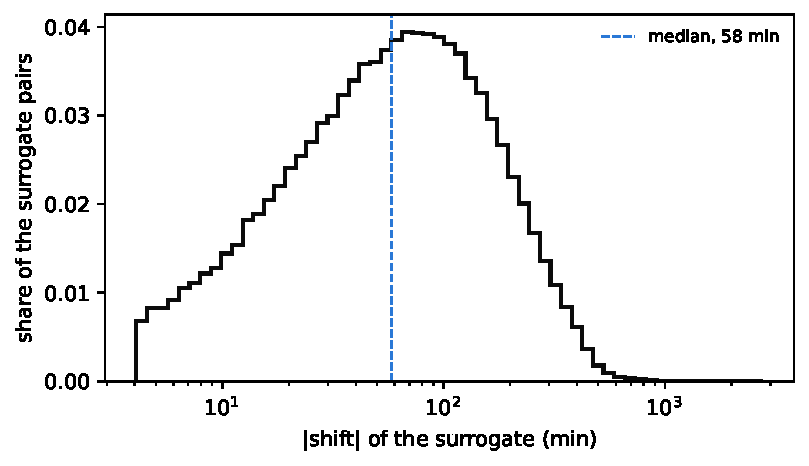
\includegraphics[width=0.62\textwidth]{figures/assessment_shifts.pdf}
\caption{The time shifts $|r_{ij}|$ of the 248\,741 surrogate pairs of the chosen run, whole
archive.}
\label{fig:shifts}
\end{figure}

\paragraph{The delay inside the contacts} (Section~\ref{sec:delta-choice}). Figure~\ref{fig:ell}
gives the whole distribution behind Table~\ref{tab:ell}: short intervals spread over the window
and pile up at its edge, long ones gather at small delays.

\begin{figure}
\centering
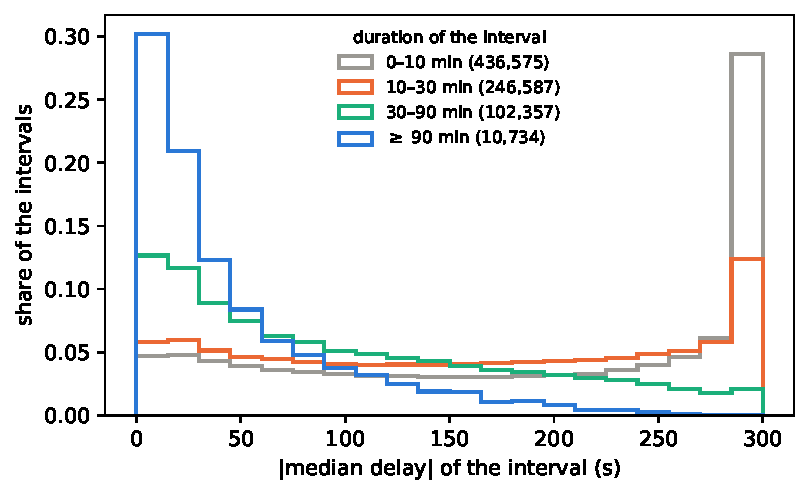
\includegraphics[width=0.62\textwidth]{figures/assessment_ell.pdf}
\caption{Distribution of the $|\ell_{\rm med}|$ of the pair intervals, by their duration
($\delta=5$~min, whole archive).}
\label{fig:ell}
\end{figure}

\paragraph{The distance at the same instant} (Section~\ref{sec:delta-choice}). Is there a distance
beyond which two pilots stop being closer than chance? We counted the distance between the two
pilots at every grid instant when both fly after departure, without requiring a correspondence,
for all the real pairs and for the surrogates, on the dates of Figure~\ref{fig:delays} that have
surrogates (210 of 300, 58\,901~h of real exposure). Real pairs are much closer than chance at
short distance and have no edge (Figure~\ref{fig:separation}): the ratio $g(d)$ is 10.4 within
100~m, below 2 from 500~m, below 1.5 from 900~m, below 1.1 from 2.7~km and below 1 from 5.7~km.
Real pairs spend 6.6\% of their time together within 1~km of each other, against 2.8\% by chance.
Beyond 6~km $g$ falls slightly below 1, because both distributions sum to one.

The excess reaches several kilometres, beyond the visual range of 1.5~km of
Section~\ref{sec:delta}. Since the surrogates also change the hour, this excess may hold the
weather of the hour as well as sight, so it bounds neither the visual range nor the range of
following.

\begin{figure}
\centering
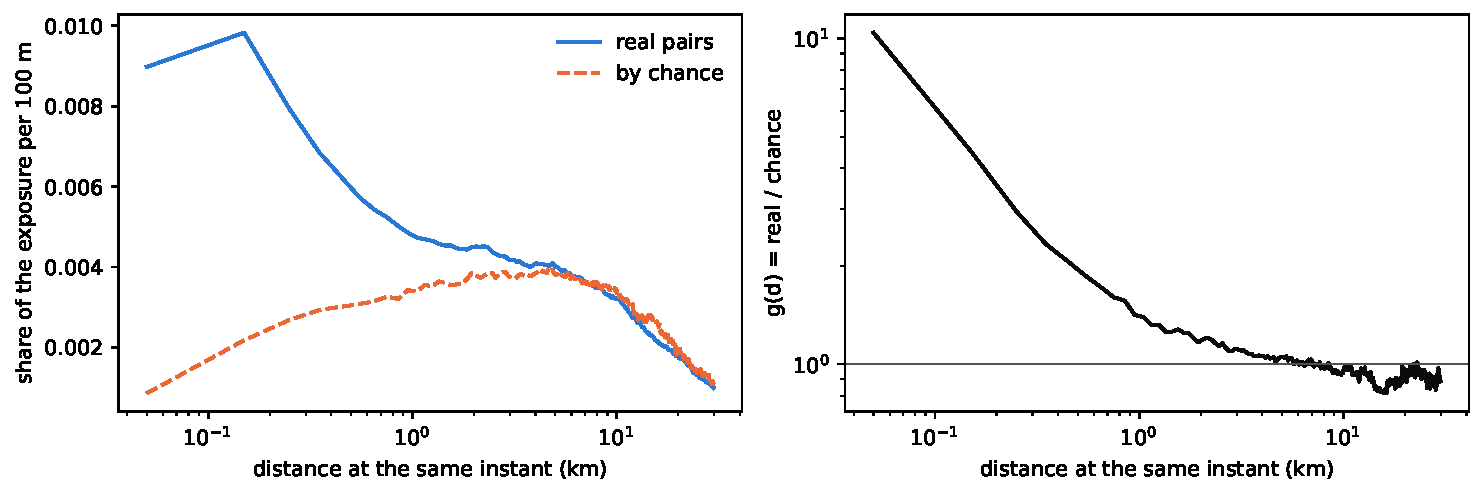
\includegraphics[width=\textwidth]{figures/assessment_separation.pdf}
\caption{Distance between the two pilots at the same instant, over all the time both fly, on
210 dates. Left: share of the exposure in each 100~m bin, real pairs and chance. Right: their
ratio $g(d)$.}
\label{fig:separation}
\end{figure}

\paragraph{One parameter at a time} (Section~\ref{sec:plateau}). Table~\ref{tab:plateau}.

\begin{table}
\centering
\small
\begin{tabular}{@{}l c c c c@{}}
\toprule
Setting ($\delta=5$ min unless stated) & $\tau^*$ (min) & $f_G$ & episodes & flights in a group \\
\midrule
starting values & 126.1 & 0.034 & 98 & 210 \\
$\varepsilon_h=250$ m & 75.1 & 0.058 & 253 & 537 \\
$\varepsilon_h=1000$ m & 126.8 & 0.065 & 162 & 372 \\
$\varepsilon_z=150$ m & 126.1 & 0.020 & 61 & 125 \\
$\varepsilon_z=600$ m & 126.1 & 0.044 & 122 & 268 \\
$\delta=2$ min & 42.6 & 0.106 & 600 & 1\,170 \\
$\delta=10$ min & 128.4 & 0.062 & 153 & 365 \\
$\theta_{\max}=30^\circ$ & 126.1 & 0.034 & 97 & 208 \\
$\theta_{\max}=90^\circ$ & 126.1 & 0.034 & 98 & 210 \\
$g=60$ s & 75.8 & 0.087 & 332 & 732 \\
$g=300$ s & 126.1 & 0.055 & 141 & 318 \\
\bottomrule
\end{tabular}
\caption{One parameter at a time on 300 random dates (7\,051 flights), $q=0.05$.}
\label{tab:plateau}
\end{table}
